\chapter{Microarchitetture}

Le micro-architetture discusse di seguito sono state ideate avendo come base i testi degli esami del corso di Ingegneria del Software nell'anno 2016. In particolare sono stati scelti tre esami fra i più adatti al tipo di elaborato in oggetto.
Tali esercizi sono stati poi modificati ed estesi, con funzionalità e nuove classi, per renderli più interessanti nelle fasi successi di analisi e testing.

\section{Termostato}

Il sistema considerato riguarda una gestione semplificata di apparecchiature di riscaldamento mediante l’uso di un termostato. 

Ciascun apparecchio si comporta in modo specifico in base allo stato in cui si trova, dipendente dalla relazione tra la temperatura da lui rilevata tramite un sensore e quella impostata dal termostato. 

Se la temperatura rilevata è inferiore a quella impostata, il sistema passa nello stato ON; se le due temperature sono equivalenti, passa nello stato READY; se la temperatura rilevata è maggiore di quella impostata passa nello stato OFF. 

In base allo stato viene poi eseguita una procedura specifica (preparazione, accensione, spegnimento).

Questa micro-architettura è stata implementata sulla base del testo di esame di Ingegneria del Software del 21 gennaio 2016, il cui testo è riportato di seguito.

\vspace{0.5cm}

\emph{Si considerino i design patterns Observer e Strategy, la cui struttura è richiamata qui di seguito:
}
\begin{figure}[h]
    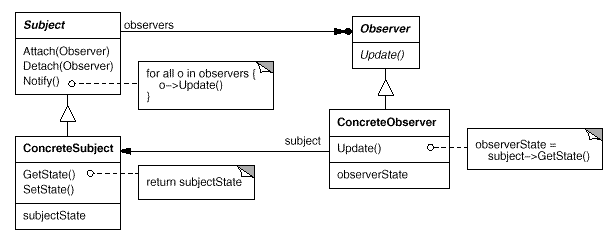
\includegraphics[scale=0.5]{../images/observer.jpg}
\end{figure}

\begin{figure}[h]
    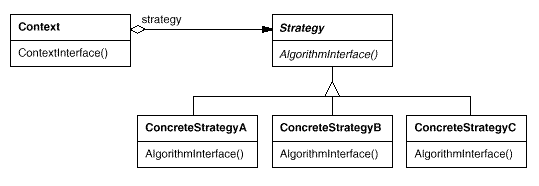
\includegraphics[scale=0.5]{../images/strategy.jpg}
\end{figure}

\emph{Si consideri uno scenario che combina i due patterns per realizzare un meccanismo di adattamento:
il Context è registrato come Observer su un qualche oggetto che opera come Monitor dell'ambiente di operazione; quando il Monitor rileva una variazione nello stato di operazione, il Context dello Strategy riceve notifica e adatta di conseguenza la Strategy con cui viene eseguita una qualche operazione.
Si descriva la struttura con cui vengono composti i due patterns, il Monitor e un Client che opera nel ruolo di test driver (il main) attraverso l'uso di un class diagram (8 punti)
Si illustri il funzionamento dello schema attraverso un sequence diagram riferito a uno scenario caratterizzante (6 punti);
Si dettaglino frammenti di codice della realizzazione che illustrano gli aspetti salienti dello schema, e si definisca uno scenario di test, realizzato per semplicità nella forma di un main(),  che esercita lo schema in no scenario che ne caratterizza l'intento (8 punti).}

\vspace{0.5cm}

Il sistema è implementato mediante l’utilizzo della combinazione di due design patterns, \emph{Observer} e \emph{Strategy}. Ciascun apparecchio rappresenta un \emph{Soggetto} che verrà monitorato da un \emph{Controller} (con la funzione di Observer). Al variare della temperatura rilevata dal \emph{Soggetto}, questa verrà notificata al suo \emph{Controllore} che andrà ad eseguire una strategia dipendente dallo stato in cui si trova il sistema.


\section{Copia difensiva}

La micro-architettura rappresenta un sistema di gestione degli esami da parte di uno studente. 

Ciascuno studente  ha un proprio libretto, in cui gli esami vengono inseriti. Il corso di laurea, utilizzando il libretto di uno studente, è in grado di calcolare la media dei voti degli esami. 

Sono previste funzionalità per il recupero e la modifica di un singolo esame, il recupero di tutti gli esami, l'aggiunta di un nuovo esame e la cancellazione di un singolo esame o di tutti gli esami presenti nel libretto di uno studente.

Questa micro-architettura è stata implementata sulla base del testo di esame di Ingegneria del Software del 17 giugno 2016, il cui testo è riportato di seguito.

\vspace{0.5cm}

\textit{Si illustri la pratica della copia difensiva nella seguente logica di dominio realizzata in Java:
}
\textit{La classe Studente ha un riferimento a un oggetto di tipo Libretto, il quale rappresenta la collezione degli Esami sostenuti dallo studente. Assumiamo che il riferimento al Libretto sia privato e che solo l'oggetto di tipo Studente che lo contiene lo possa modificare.}

\textit{La classe CorsoDiLaurea espone:
\begin{itemize}
\item un metodo getMedia(Libretto lib) che riceve il riferimento a un Libretto e calcola la media secondo le regole del particolare corso di laurea.
\end{itemize}}


\textit{La classe Studente espone:
\begin{itemize}
\item un metodo costruttore Studente(Libretto lib) che riceve come parametro un riferimento a un Libretto già inizializzato e che ha la responsabilità di creare l'oggetto di Studente componendo al suo interno l'oggetto di tipo Libretto;
\item un metodo pubblico getMedia(CorsoDiLaurea cdl) che riceve come parametro un riferimento a un oggetto di tipo CorsoDiLaurea e realizza il metodo per forwarding invocando il metodo getMedia sul corso di laurea.
\end{itemize}}


\textit{Si realizzi una descrizione UML della logica di domino (5 punti).
Si motivi la convenienza di realizzare una copia difensiva al momento della creazione di un oggetto di tipo Studente e al momento della invocazione del metodo getMedia sull'oggetto di tipo Studente (8 punti).}

\textit{Si riportino frammenti di codice che illustrano i tratti salienti dell'implementazione (10 punti.) }

\vspace{0.5cm}

Il sistema è implementato utilizzando la tecnica della \emph{copia difensiva}, ovvero invece di condividere l'oggetto originale, nel caso di studio il libretto o l'esame, viene condivisa una copia di esso, in modo da limitare gli effetti negativi di modifiche inattese.


\section{Generatore di espressioni booleane}

Il sistema considerato riguarda la creazione di espressioni booleane, potendo combinare fra di loro variabili booleane, operatori logici quali AND, OR, NOT e l'uso di parentesi.

Esso è in grado di valutare correttamente tali espressioni booleane e di stamparle a schermo, mostrando il valore assegnato alle singole variabili più la valutazione finale dell'intera espressione.

Questa micro-architettura è stata implementata sulla base del testo di esame di Ingegneria del Software del 26 febbraio 2016, il cui testo è riportato di seguito.

\vspace{0.5cm}

\textit{Si considerino i design patterns Composite e Builder.}

\begin{figure}[h]
    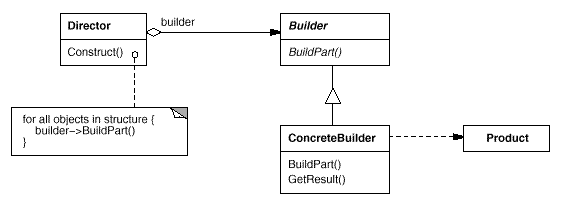
\includegraphics[scale=0.5]{../images/builder.jpg}
\end{figure}

\begin{figure}[h]
    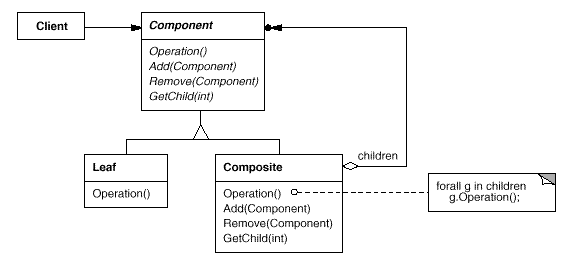
\includegraphics[scale=0.5]{../images/composite.jpg}
\end{figure}

\textit{Si consideri uno scenario che combina i due patterns per costruire e rappresentare
un'espressione Booleana:
\begin{itemize}
\item lo schema del Composite viene applicato per rappresentare e valutare un'espressione
Booleana nella quale un insieme di variabili possono essere combinate attraverso i
connettivi AND e OR e attraverso l'operatore di parentesi ().
[Suggerimento: le variabili sono rappresentate come istanze di Leaf, i connettivi AND,
OR e la parentesi ()sono rappresentati come istanze di subclassi di Composite.]
\item Lo schema del Builder viene applicato per costruire il Composite che rappresenta una
assegnata espressione.
[Suggerimento: il Builder espone i metodi per costruire una variabile, un AND, un OR
e una parentesi(); tali metodi restituiscono un riferimento a un Product, che nel caso
specifico è un Component; il Director tiene memoria dei Components messi in vita e li
usa per passarli al metodo di costruzione di ciascun Component]
\end{itemize}}


\textit{Si consideri in particolare lo scenario in cui il Builder mette in vita il Composite che
rappresenta l'espressione (X AND Y) Or Z, e in riferimento a questo caso:
\begin{itemize}
\item Si descriva la struttura con cui vengono composti i due patterns attraverso l'uso di un
class diagram (11 punti).
\item Si illustri il funzionamento dello schema attraverso un object diagram che
rappresenta gli oggetti messi in vita nella rappresentazione dell'espressione e quelli
usati per metterli in vita (8 punti);
\item Si dettaglino frammenti di codice della realizzazione che illustrano aspetti salienti
dello schema, e si definisca uno scenario di test, realizzato per semplicità nella forma
di un main(), che esercita lo schema in uno scenario che ne caratterizza l'intento (11
punti).
\end{itemize}}

\vspace{0.5cm}

Il sistema è implementato combinando i design patterns \emph{Composite} e \emph{Builder}. Il design pattern \emph{Composite} definisce le interfacce per creare le componenti semplici, le variabili, e le componenti composte, gli operatori e le parentesi. Il design pattern \emph{Builder} si occupa di istanziare correttamente tali componenti e di combinarle fra di loro per creare delle espressioni booleane più complesse.
